\documentclass[nocover]{pset}
\usepackage{tikz-cd}
\pagestyle{fancy}
\fancyhf{}
\lhead{Forest Kobayashi}
\chead{Basic Category Theory}
\rhead{Math 196 -- Fall, 2018}
\rfoot{\thepage\ of \pageref{LastPage}}
\setlength{\headheight}{15.2pt}
\setlength{\headsep}{10pt}
\lfoot{Friday, October 18th 2018}

\usepackage[normalem]{ulem} % [normalem] prevents the package from
                            % changing the default behavior of `\emph`
                            % to underline.

\titleformat{\section}
  {\LARGE \scshape}{\thesection.}{.5em}{\vspace{.5em}}

\titleformat{\subsection}
  {\Large \scshape}{\thesubsection.}{.5em}{}

\tikzstyle{titlerule}=[dash pattern=on \pgflinewidth off 2pt]
\usetikzlibrary{decorations.markings}

\newcommand{\wah}[1]{
  \tikz[decoration={markings, mark=between positions 0 and 1 step 3pt
    with { \draw [fill] (0,0) circle [radius=.5pt];}},
  baseline=(todotted.base)]{
  \node[inner sep=0pt,outer sep=0pt] (todotted) {#1};
  \path[postaction={decorate}] (todotted.south west) --
  (todotted.south east);}
}

\newcommand{\udot}[1]{%
    \tikz[baseline=(todotted.base)]{
        \node[inner sep=1pt,outer sep=0pt] (todotted) {#1};
        \draw[titlerule] (todotted.south west) -- (todotted.south east);
    }%
}%

\usepackage{upgreek}

\usetikzlibrary{
  knots,
  hobby,
  decorations.pathreplacing,
  shapes.geometric,
  calc
}

\tikzset{
  knot diagram/every strand/.append style={
    ultra thick,
    blue
  },
  show curve controls/.style={
    postaction=decorate,
    decoration={show path construction,
      curveto code={
        \draw [blue, dashed]
        (\tikzinputsegmentfirst) -- (\tikzinputsegmentsupporta)
        node [at end, draw, solid, blue, inner sep=2pt]{};
        \draw [blue, dashed]
        (\tikzinputsegmentsupportb) -- (\tikzinputsegmentlast)
        node [at start, draw, solid, blue, inner sep=2pt]{}
        node [at end, fill, blue, ellipse, inner sep=2pt]{}
        ;
      }
    }
  },
  show curve endpoints/.style={
    postaction=decorate,
    decoration={show path construction,
      curveto code={
        \node [fill, red, ellipse, inner sep=2pt] at (\tikzinputsegmentlast) {}
        ;
      }
    }
  }
}

\usepackage{caption}

\begin{document}

\begin{center}
  {\scshape \Large Basic Algebraic Topology}

  {\itshape Based on Kosniowski; Matveev}
\end{center}
\vspace{-.1cm}
\hrulefill
\section{Introduction}
\begin{adjustwidth}{1em}{1em}
  First, a motivating quote.
  \begin{quote}
    ``Point set topology is a disease from which later generations
    will regard themselves as having recovered'' -Henri Poincar\'{e}
  \end{quote}
  That's\ldots not exactly a ringing endorsement. Why did Henri
  Poincar\'{e} have such a low opinion of point-set topology? Well,
  loosely speaking, because it's just not the right tool for the job,
  especially when compared to \emph{algebraic topology}.

  As it turns out, lots of topics in topology can be simplified by
  attaching algebraic objects to topological spaces, and proving that
  certain properties of this object correspond naturally to properties
  of our topological space. The vehicle by which we navigate between
  the two is, as one might expect, Category Theory. First, we give a
  brief summary of basic concepts in algebraic topology, before moving
  into the Homology presentation given in Matveev.

  \subsection{Basic Point-Set Topology}
  As in most branches of mathematics, our object of study here will be
  some collection of sets, together with some \emph{structure} we can
  associate with them. In Elementary Algebra, this takes the form of
  \emph{group} and \emph{ring} operations, and later the respective
  homomorphisms preserving them. In Elementary Analysis, this (loosely
  speaking) took the form of a \emph{distance metric}, and the
  properties it bestowed on sets. Analogous to our study of
  homomorphisms in Algebra, we often studied \emph{continuous
    functions} in Analysis, and the properties of sets that they
  preserved. Note the resemblance between the two expressions:
  \begin{minipage}[H]{.49\linewidth}
    \begin{figure}[H]
      \centering
      \[
        \varphi(g_1 \oplus g_2) = \varphi(g_1) \otimes \varphi(g_2)
      \]
      \caption*{A homomorphism $\varphi : G \to H$}
    \end{figure}
  \end{minipage}
  \begin{minipage}[H]{.49\linewidth}
    \begin{figure}[H]
      \centering
      \[
        d(x,y) < \delta \implies d'(f(x), f(y)) < \varepsilon
      \]
      \caption*{A continuous function $f : (E,d) \to (E', d')$}
    \end{figure}
  \end{minipage}

  while the analogy doesn't hold exactly, in both cases, we have some
  particular class of functions such that structure in one space is
  preserved in the image. In the case of homomorphisms, the group
  operation in the first group is ``respected'' by the homomorphism
  upon mapping into the second. In the case of continuous functions,
  our equation is essentially stating that the function respects
  things being ``close'' to one another (our map doesn't destroy the
  properties of the distance metric). We can think of this as
  stipulating that we didn't ``tear'' our starting space at all. This
  is best visualized by thinking about our continuous functions not as
  their \emph{graphs} (as we are often used to), but rather as
  \emph{maps} that deform the input domain in various manners to yield
  the image. As an example, one might think of the function $f(x) =
  x^2$ as the action of folding $\RR$ on itself, and stretching the
  edges out towards infinity (this is often a strategy employed in
  visualizing complex-valued functions).

  One might wonder what sorts of interesting discoveries we could make
  by generalizing our starting premises on the right-hand-side, so
  that we could make our questions more similar to those on the left.
  That is, similarly to how we defined distance metrics so as to
  generalize the \emph{key} properties of Euclidean distance, so too
  will we generalize the idea of \emph{continuity of a function}. This
  is the central idea of basic topology. Now, all we need is a good
  place to start. Recall the following theorem of Analysis:
  \begin{theorem}
    Let $(E,d)$ and $(E', d')$ be metric spaces. Then a function $f :
    E \to E'$ is said to be \emph{continuous} iff for all open sets $U
    \subseteq M_2$, we have $f^{-1}(U) \text{ is open in } M_1$.
  \end{theorem}
  Note, this theorem makes no guarantees about the image of an open
  set being open in the codomain. Really, we can make our image as
  ``jagged'' as we want (within reason), provided we fold and deform
  our domain in a smooth manner. But it does indicate to us open sets
  appear to be intimately tied to the idea of ``smooth'' deformations.
  In particular, noting that the theorem is an if and only if, we
  might wonder what would happen were we to discard the distance
  metric entirely, and take the above as a \emph{definition} instead
  of as a \emph{theorem}. There's just one catch: if we really want to
  discard the metric, how are we going to define the notion of an
  ``open'' set? Topologies provide the answer.
  % --- and that it might be fruitful to pursue an understanding of our
  % space that does not depend on the details of a particular metric,
  % but rather just on relationships between open sets.

  % Hence, we define
  % a topology as follows:
  \begin{definition}
    Let $X$ be a set, and let $\mc U$ be a collection of subsets of
    $X$ satisfying the following:
    \begin{enumerate}[label=(\roman*)]
      \item $\varnothing \in \mc U$, $X \in \mc U$.
      \item For all $U_1, U_2 \in \mc U$, we have $U_1 \cap U_2 \in
        \mc U$ (by induction, we obtain closure under finite
        intersections).
      \item For any subset $\set{U_i \mid i \in I} \subseteq \mc U$,
        we have
        \[
          \bigcup_{i \in I} U_i = \bm{U} \in \mc U
        \]
        ($\mc U$ is closed under arbitrary unions).
    \end{enumerate}
    then $\mc U$ is called a \emph{topology} for $X$, and $(X, \mc U)$
    is called a \emph{topological space}. We call the elements of $\mc
    U$ the \emph{open sets of} $(X, \mc U)$.
  \end{definition}
  note that a topology is thus a particular kind of \emph{algebra of
    sets} under the binary operations $\cup, \cap$, with identity
  $\varnothing$ for $\cup$, and $X$ for $\cap$. Note that $(\cup,
  \varnothing)$, $(\cap, X)$ are duals of each other, in the sense
  that for any sentence $S$ built out of atomic propositions about our
  set algebra, if $S$ is true, then the statement we obtain by
  \begin{enumerate}[label=\arabic*.]
    \item Replacing each $\cup$ with $\cap$ and each $\cap$ with
      $\cup$,
    \item Interchanging each $\varnothing$ and $X$, and
    \item Reversing inclusions
  \end{enumerate}
  must also be true. Less relevantly (but maybe an object of
  interest), observe that if we replace ``arbitrary unions'' with
  ``countable unions'', and further require closure under
  complementation, then we obtain a $\sigma$-algebra.

  As it turns out, this definition of a topology is more general than
  that given by distance metrics. Whereas every distance metric gives
  rise to a topology, there are topologies that are not
  \emph{metrizable}, meaning they do not arise from any metric on a
  set. We list a few common topologies. Let $(X, \mc U)$ be a
  topological space. Then
  \begin{enumerate}[label=\arabic*.]
    \item If $\mc U = \set{\varnothing, X}$, we call $\mc U$ the
      \emph{concrete} or \emph{indiscrete topology}.
    \item If $\mc U = \mc P(X)$ (i.e., every subset of $X$ is open),
      then we call $\mc U$ the \emph{discrete topology}. Note the
      direct connection to the discrete metric.
    \item Suppose $\mc U = \set{\varnothing, X} \cup \set{U \subseteq
        X \MID \abs{\ol{U}} < \infty}$. That is, $X, \varnothing$, and
      all subsets of $X$ with finite compliment. Then call $\mc U$ the
      \emph{finite complement topology}.
    \item Let $X = \RR$, and $\mc U = \set{\varnothing, \RR} \cup
      \set{(x, \infty) \MID x \in \RR}$
  \end{enumerate}
  As an exercise, I'll give a proof for some of these. Note that
  below, I'll be using overline to denote the compliment of a set, a
  notation I'll discard quickly once we start talking about
  compliments. But for now, it's the most convenient.
  \begin{enumerate}[label=\arabic*.]
    \item Trivial
    \item Also trivial
    \item Observe $\varnothing, X \in \mc U$ by definition. We first
      prove that $\mc U$ is closed under finite intersections. Let
      $U_1, U_2 \in \mc U$. Then $\ol{U_1 \cap U_2} = \ol{U_1} \cup
      \ol{U_2}$ (De Morgan's Laws). The union of two finite sets is
      finite, hence $\ol{U_1 \cap U_2}$ is finite and so $U_1 \cap U_2
      \in \mc U$. Now, let $U' = \set{U_i \mid i \in I} \subseteq \mc
      U$. Then
      \begin{align*}
        \ol{\bigcup_{i \in I} U_i}
        &= \bigcap_{i \in I} \ol{U_i}
      \end{align*}
      which is an intersection of finite sets, and is thust finite
      itself. Hence $\mc U$ is closed under arbitrary unions. It
      follows that $(X, \mc U)$ is a topological space. \qed
    \item The non-trivial elements of $\mc U$ inhereit a total order
      by inclusion from the total order on $\RR$. We add $\varnothing,
      \RR$ to the total order by putting $\RR = \sup (\mc U)$,
      $\varnothing = \inf (\mc U)$. The closure properties follow.
      \qed
  \end{enumerate}
  We define some noteworthy sets.
  \begin{definition}[Interior]
    Let $(X, \mc U)$ be a topological space. Let $Y \subseteq X$. Let
    $U' = \set{U_i \in \mc U \mid i \in I, U_i \subseteq Y}$ be the
    set of all open sets contained in $Y$. Then call the
    \emph{interior} of $Y$ (sometimes denoted $Y^\circ$)
    \[
      \mrm{int}(Y) = \bigcup_{i \in I} U_i.
    \]
  \end{definition}
  we have open sets --- what's next, closed sets???? Yeah, uh, you got
  me there.
  \begin{definition}[Closed sets]
    Let $(X, \mc U)$ be a topological space. Let $C \subseteq X$, and
    let $X - C$ denote the compliment of $C$ in $X$. Then call $C$
    \emph{closed} iff $X - C$ is open. \textbf{VERY VERY IMPORTANT:}
    a set can be both open and closed. In fact, in the discrete
    topology, every set is both.
  \end{definition}
  From the principle of duality (or, alternatively, De Morgan's Laws),
  the dual statements of the topology axioms hold for closed sets.
  That is,
  \begin{enumerate}[label=\roman*.]
    \item $X, \varnothing$ are closed
    \item The set of closed sets is closed (haha) under finite unions
    \item The set of closed sets is closed under arbitrary
      intersections
  \end{enumerate}
  Analogously to the interior of a set, we define its closure. Note
  closure is, in a sense, the dual of the interior
  operator. \clearpage
  \begin{definition}
    Let $(X, \mc U)$ be a topological space. Let $Y \subseteq X$. Then
    let
    \[
      V' = \set{V_i \mid i \in I, X - V_i \in \mc U, Y \subseteq V_i}
    \]
    that is, the set of all closed sets containing $Y$. Then call the
    \emph{closure} of $Y$ (denoted $\ol{Y}$)
    \[
      \mrm{clos}(Y) = \bigcap_{i \in I} V_i
    \]
  \end{definition}
  Finally, we define the boundary of a set as
  \begin{definition}
    Let $(X, \mc U)$ a topological space. Let $Y \subseteq X$. Then
    define the boundary of $Y$, denoted $\partial Y$, by $\partial Y =
    \ol{Y} - Y$.
  \end{definition}
  One might wonder why we've chosen to recycle the partial derivative
  notation to denote the boundary. The intuitiion is as follows (this
  lightly paraphrased from a stackexchange answer by Terry Tao):
  \begin{leftbar}
    Let $S$ be a smooth, bounded body. Then the surface area
    $\abs{\partial S}$ is the derivative of the volume $\abs{S_r}$ of
    the $r$-neighborhoods $S_r$ at $r = 0$:
    \[
      \abs{\partial S} = \od{}{r} \abs{S_r} \bigg\vert_{r=0}
    \]
    Here's the part I don't understand: he then goes on to say ``More
    generally, one intuitively has the Newton quotient-like formula''
    \[
      \partial S = \lim_{h \to 0^+} \frac{S_h \setminus S}{h}
    \]
    ``the right-hand side does not really make formal sense, but
    certainly one can view $S_h \setminus S$ as a $[0,h]$-bundle over
    $\partial S$ for $h$ sufficiently small (in particular, the radius
    of curvature of $S$).''
  \end{leftbar}
  Finally, we define the neighborhood of a point $x$.
  \begin{definition}[Neighborhood]
    Let $(X, \mc U)$ be a topological space. Let $N \subseteq X$, and
    let $x \in N$. Then call $N$ a neighborhood of $x$ if $x \in
    N^\circ$.
  \end{definition}
  Note the following properties:
  \begin{enumerate}[label=\arabic*.]
    \item $\mrm{clos}$ and $\mrm{int}$ are idempotent.
    \item $X - Y^\circ = \ol{X - Y}$
    \item $\partial Y = \varnothing \iff Y$ is clopen.
    \item Let $U \in \mc U$. Then $Y = \ol{U} \iff Y = \ol{U^\circ}$
      (proof: note $U = U^\circ$).
    \item For each point $x \in X$, there is at least one neighborhood
      of $x$, namely $X$.
    \item If $M$ and $N$ are neighborhoods of $x$, then so is $N \cap
      M$ (use closure under finite intersections).
  \end{enumerate}
  \subsection{Continuous functions and Induced Topologies}
  As promised, we'll now define a continuous function between two
  topological spaces.
  \begin{definition}[Continuous Function]
    A function $f : X \to Y$ between two topological spaces is said to
    be \emph{continuous} if for every open set $U \subset Y$, the
    inverse image $f^{-1}(U)$ is open in $X$ (the same holds for
    closed sets). These are the morphisms in \textbf{Top}.

    If $f$ is bijective with a continuous inverse, then call $f$ a
    \emph{homeomorphism}.
  \end{definition}
  Question: how can we make the following into a trivial statement of
  category theory?
  \begin{leftbar}
    Let $Y$ be a topological space with the property that for every
    topological space $X$, all functions $f : X \to Y$ are continuous.
    Prove that $Y$ has the concrete topology.
  \end{leftbar}
  Answer: use the forgetful functor and the universal mapping
  principle?
  \begin{definition}[Open / closed maps]
    Let $f : X \to Y$. If the image of every open set is open, $f$ is
    said to be \emph{an open map} (define closed maps analogously).
    Note, open mappings are not necessarily continuous.
  \end{definition}
  And lastly, a convenient theorem.
  \begin{theorem}
    Let $(X, \mc U)$, $(Y, \mc V)$ be topological spaces, with $X
    \cong Y$ by a homemorphism $h : X \to Y$. Then for every point $x
    \in X$, $X - \set{x} \cong Y - \set{h(x)}$ (that is, removing a
    point preserves the homeomorphism).
  \end{theorem}
  Intuitively, we think of homeomorphisms as encoding information
  about how two spaces can be stretched and deformed into one another,
  without tearing / gluing pieces together / apart. Note, however,
  that this does not necessarily correspond to our intuitive
  understanding of ``tearing / gluing'' --- were I to hand you a
  circular segment of rope, and ask you to construct the following
  knot
  \begin{figure}[H]
    \centering
    \begin{tikzpicture}
      \begin{knot}[
        consider self intersections=true,
        % draft mode=crossings,
        flip crossing/.list={2,4},
        only when rendering/.style={
          % show curve controls
        }
        ]
        \strand (2,0) .. controls +(0,1.0) and +(54:1.0) .. (144:2) ..
        controls +(54:-1.0) and +(18:-1.0) .. (-72:2) .. controls
        +(18:1.0) and +(162:-1.0) .. (72:2) .. controls +(162:1.0) and
        +(126:1.0) .. (-144:2) .. controls +(126:-1.0) and +(0,-1.0)
        .. (2,0);
      \end{knot}
      % \begin{knot}[
      %   consider self intersections=true,
      %   % draft mode=crossings,
      %   flip crossing/.list={2,4,6}
      %   ]
      %   \strand ([closed]90:2) foreach \k in {1,...,7} { .. (90-360/7+\k*720/7:1.5) .. (90+\k*720/7:2) } (90:2);
      % \end{knot}
    \end{tikzpicture}
    \caption{cinquefoil}
  \end{figure}
  you'd say it couldn't be done. However that's not exactly true. If
  we weren't constrained by the pesky physical details of the real
  world, we could simply pass the rope through itself to yield the
  desired knot. This is what is meant in topology by a homeomorphism
  --- all that has to be conserved are, loosely speaking,
  ``adjacency'' relationships. On the flip side, we might also note
  that this knot can hardly be said to ``not differ at all'' from a
  circle. But in a topological sense, they are homeomorphic. Maybe
  we'll talk about ambient isotopy next week.

  Now, induced topologies. Loosely speaking, this works kind of like a
  group action, except by a topological space on a subset of the
  underlying set. It's worth noting that this analogy might be
  \emph{highly} tenuous.
  \begin{definition}[Induced topologies]
    Let $(X, \mc U)$ be a topological space, and $S \subseteq X$. Let
    $\mc U' = \set{U \cap S \MID U \in \mc U}$. Then we call $\mc U'$
    \emph{the topology on $S$ induced by the topology of $X$} (note
    the desired topological axioms follow from the properties of $\mc
    U$ and the commutativity of union / intersection on sets). If $S$
    has the induced topology, we call $S$ a subspace of $X$.
  \end{definition}
  One thing to note about this definition is that an open set in the
  induced topology need not be open in the original topology. Really,
  what we've essentially done is ``project'' the topological structure
  of some space on to one of its subsets. Naturally, this can't give
  us information about the open-ness of a set selected from $\mc U'$
  were we to imbed it back into $\mc U$. However, if we do know
  something about how $S$ is related to $X$ from the get go,
  \emph{then} we can guarantee a stronger condition:
  \begin{theorem}
    If $S \in \mc U$, then $\mc U' \subseteq \mc U$. That is, the
    opens sets of $S$ are open in $X$. The proof follows directly from
    the definition of induced topology.
  \end{theorem}
  \subsection{Quotient Topology}
  Whereas the induced topology can be thought of as arising from an
  injetive map $\iota : S \to X$, we will now consider the topology
  arising from a surjective map $q : X \to Y$.
  \begin{definition}[Quotient topology]
    Let $f : (X, \mc U) \to Y$ be surjective as a function of sets.
    Then define the \emph{quotient topology} on $Y$ by
    \[
      \mc U' = \set{U \subseteq Y \MID f^{-1}(U) \in \mc U}.
    \]
    The topology axioms follow from properties of the inverse image.
    Once $Y$ has been endowed with the quotient topology, $f$ becomes
    a continuous map.
  \end{definition}
  \begin{theorem}
    Let $f : X \to Y$ be a mapping and suppose that $Y$ has the
    quotient topology with respect to $X$. Let $Z$ be a topological
    space. Then a mapping $g : Y \to Z$ is continuous iff $gf$ is
    continuous.
  \end{theorem}
  In our definition of a quotient topology, because $Y$ is a set
  intially without structure, we don't really care what exactly its
  elements are --- really, all that matters to us is that our mapping
  is surjective ($Y$ only assumes structure once we define the
  quotient topology). Hence, there's no reason why we can't treat all
  such $Y$ as if they were subsets of $X$ (every surjective mapping
  from $X$ to $Y$ can be factored through an isomorphism of $Y$ with a
  subset of $X$). This, together with the suspicious name ``quotient
  topology,'' leads us to question whether we can view this as some
  form of \emph{mod} operation. Indeed, we can. Recall the standard
  definition of an equivalence relation: \clearpage
  \begin{definition}
    Let $X$ be a set. Then an \emph{equivalence relation} $\sim$ is a
    binary relation such that
    \begin{enumerate}
      \item $\sim$ is reflexive,
      \item $\sim$ is symmetric, and
      \item $\sim$ is transitive.
    \end{enumerate}
    For each $x \in X$, we define the \emph{equivalence class of $x$}
    under $\sim$ by $[x] = \set{y \in X \MID x \sim y}$. The set of
    equivalence classes of $X$ under $\sim$ is usually denoted
    $X/\sim$.
  \end{definition}

  % It is easy to verify that for $(X,\mc U)$ a topological space, $Y$ a
  % set, and $f : X \to Y$, $f$ defines an equivalence relation by $f(x)
  % = [x]$
\end{adjustwidth}

\end{document}
